\documentclass[a4paper,12pt]{article}
\usepackage[T1]{fontenc}
\usepackage{ninecolors}
\usepackage{booktabs}
\usepackage{caption}
\usepackage{tabularray}
\usepackage{hyperref}
\usepackage{graphicx}
\usepackage{subcaption}
\usepackage{parskip}
\usepackage{float}
\hypersetup{
  colorlinks=true,
  linkcolor=blue,
  filecolor=magenta,
  urlcolor=cyan,
  pdftitle={Lizard Kisses},
  pdfpagemode=FullScreen,
}
\graphicspath{ {img/} }
\captionsetup[table]{position=bottom}
\usepackage{geometry}
\usepackage{siunitx}
\usepackage{awesomebox}

\begin{document}
\begin{titlepage}
  \vspace*{\stretch{1.0}}
  \begin{center}
    \Large\textbf{Lizard Kisses}\\
    \large{Overdrive pedal kit by Pedal Markt}
  \end{center}
  \vspace*{\fill}
  \begin{center}
    \today
  \end{center}
\end{titlepage}

\tableofcontents
\pagebreak

\section{Introduction}
Lizard Kisses is a color and texture device. With different
clipping and brightness options it can act as a boost, an
overdrive or a distortion. It stacks well with other pedals,
responds to your playing and is a classy beast all around!

Lizard Kisses enclosure was designed by the wonderful
\href{https://fiz.gallery/}{Agata Fiz.}

\begin{figure}[h!]
  \centering
  \begin{subfigure}[b]{0.49\textwidth}
    \centering
    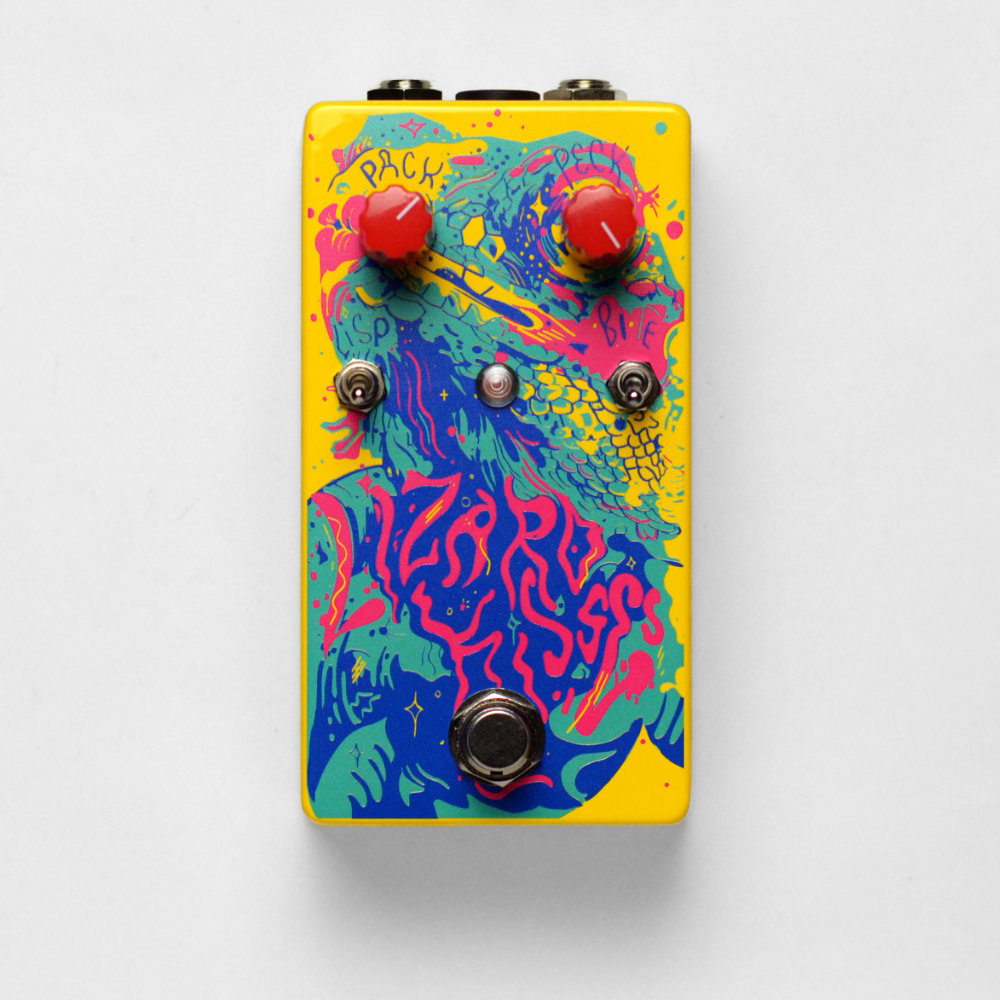
\includegraphics[width=\textwidth]{lizard-kisses-1000px.jpg}
  \end{subfigure}
  \begin{subfigure}[b]{0.49\textwidth}
    \centering
    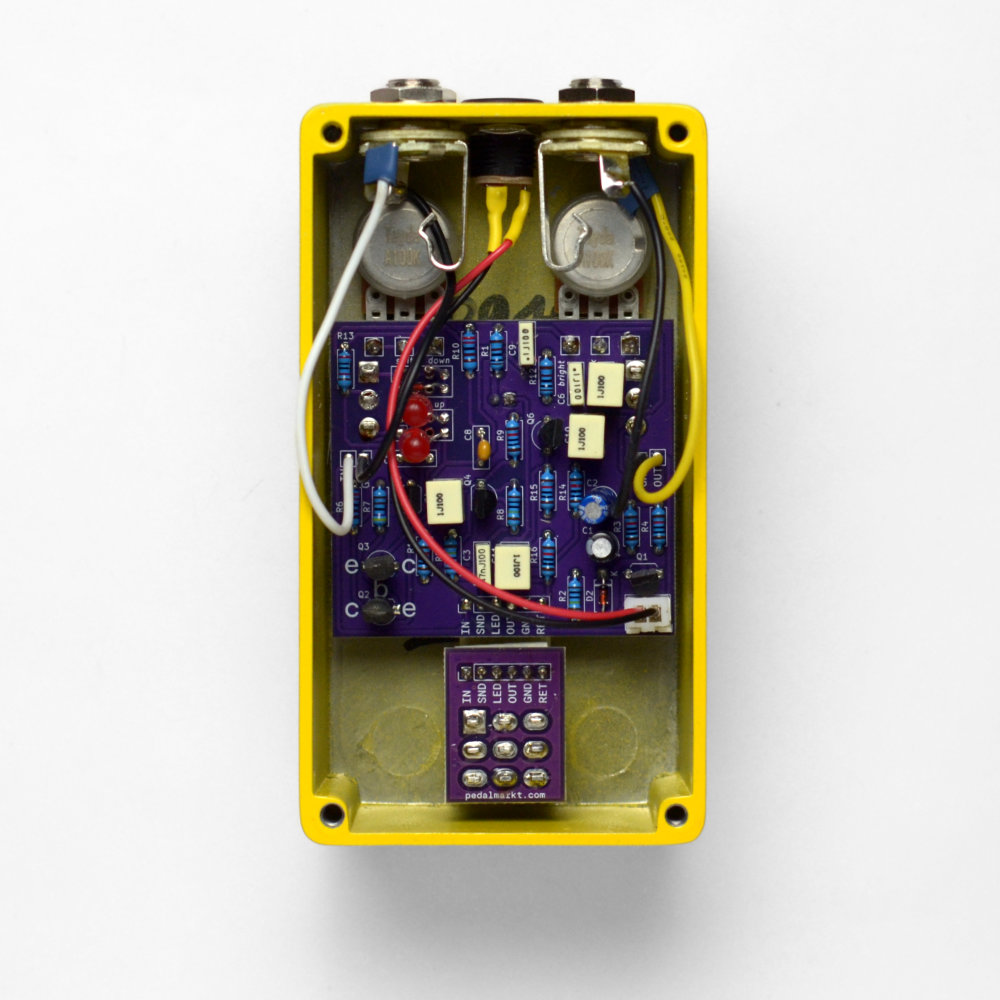
\includegraphics[width=\textwidth]{lizard-kisses-inside-1000px.jpg}
  \end{subfigure}
  \caption{Lizard Kisses: oustide and inside}
  \label{fig:lk}
\end{figure}

The pedal was originally conceived for the workshops at
\href{https://pedalmarkt.com}{Pedal Markt.} The intention
was  to make it as easy to build and customize as possible.
The \hyperref[sec:bom]{BOM} lists the stock values for
components, and separate sections further in the document
describe how you could try out alternative parts to get
different sounds.

The circuit is based around a discrete operational
amplifier. Discrete meaning it's built out of single
transistors, as opposed to an integrated circuit aka a chip.
You can find \hyperref[sec:schematic]{the schematic} and
\hyperref[sec:circuit]{the circuit breakdown} further in the
document.

\pagebreak

\section{BOM – Bill of Materials}
\label{sec:bom}

BOM is a document that lists the parts you'd need to build a
project. Each row corresponds to a component with a certain
value, for example a `ceramic capacitor with value 1nF.`
There could be one or more actual physical part per each
row, their designators are listed in the \textit{Reference}
column.

\tipbox{
  Components in the BOM are listed in order of assembly. Go
  through the table top to bottom.

  If you haven't built a kit before, check out the
  \hyperref[sec:steps]{Step-by-step instructions} first.
}

\tipbox{
  In the BOM \textit{text in italic font} gives tips about how to mount or
  solder parts.
}

\tipbox{
  If you'd like to experiment with some of the parts, for
  example the Brightness Caps and the Clipping Diodes, please
  socket them.
}

\newgeometry{hmargin={1cm}}

\begin{longtblr}[caption = {BOM}]{
  hlines,
  vlines,
  rows={ht=1.2em},
  row{even}={bg=gray9},
  row{1}={bg=gray3,fg=white},
  width=\linewidth,
  colspec={lX[1]llX[2]},
}
  \hspace{1em}
  & \textbf{Ref}
  & \textbf{Value}
  & \textbf{Qnty}
  & \textbf{Description}
  \\
  \SetCell[c=5]{c,bg=gray6,fg=white}\textbf{Outboard}
  \\
  \hspace{1em}
  & -- & Enclosure & 1 & \textit{Mount both pots, both
  toggle switches, DC jack, Footswitch and LED Lampshade
  into the enclosure before soldering}
  \\
  \hspace{1em}
  & -- & Lampshade & 1
  & Small transparent plastic part for the LED,
  \textit{mount in enclosure before putting the boards in}
  \\
  \hspace{1em}
  & -- & Rubber Ring & 1
  & \textit{Use it to keep LED Lampshade in place}
  \\
  \hspace{1em}
  & -- & DC Jack & 1
  & Black plastic part with a nut, \textit{mount in
  enclosure before soldering}
  \\
  \hspace{1em}
  & -- & DC Cable & 1
  & Red and black cables in a JST connector, \textit{cut to
  $\approx12cm$ and solder to DC Jack once it's mounted in enclosure}
  \\
  \hspace{1em}
  & -- & Audio Jack & 2 & \textit{Only mount these in the
  enclosure together with the main board once they are wired up}
  \\
  \SetCell[c=5]{c,bg=gray6,fg=white}\textbf{Main board, floor side}
  \\
  \hspace{1em}
  & GND & Wire & 2 & $\approx10cm$, black, \textit{strip and
  tin the ends}
  \\
  \hspace{1em}
  & IN & Wire & 1 & $\approx10cm$, any color, \textit{strip and tin
  the ends}
  \\
  \hspace{1em}
  & OUT & Wire & 1 & $\approx10cm$, any other color,
  \textit{strip and tin the ends}
  \\
  \hspace{1em}
  & R7 & 4.7k & 1 & Resistor
  \\
  \hspace{1em}
  & R13 & 20k & 1
  & Resistor
  \\
  \hspace{1em}
  & R1 & 1k & 1
  & Resistor for the LED, \textit{larger value will make the LED
  dimmer, values up to 6.8k are reasonable}
  \\
  \hspace{1em}
  & R12 & 1k & 1
  & Resistor
  \\
  \hspace{1em}
  & R6, R10 & 2.2k & 2
  & Resistor
  \\
  \hspace{1em}
  & R2, R5, R8 & 1M & 3
  & Resistor
  \\
  \hspace{1em}
  & R3, R4, R9, R11, R14, R15, R16 & 10k & 7
  & Resistor
  \\
  \hspace{1em}
  & D2 & 1N4148 & 1
  & Diode, orientation matters
  \\
  \hspace{1em}
  & switch up & 1N4148 & 3
  & See \hyperref[sec:clip]{Clipping Diodes} section
  \\
  \hspace{1em}
  & Q1 & TP0606 & 1
  & P-channel MOSFET
  \\
  \hspace{1em}
  & Q5 & 2N3906 & 1
  & PNP transistor
  \\
  \hspace{1em}
  & Q2, Q3, Q4, Q6 & 2N3904 & 4
  & NPN transistor
  \\
  \hspace{1em}
  & C5, C8 & 47p & 2
  & Ceramic capacitor
  \\
  \hspace{1em}
  & C3 & 47n & 1
  & Film capacitor
  \\
  \hspace{1em}
  & C9 & 100n & 1
  & Film capacitor
  \\
  \hspace{1em}
  & C6 (bright) & 330n & 1
  & See \hyperref[sec:caps]{Brightness capacitors} section
  \\
  \hspace{1em}
  & C7 (dark) & 470n & 1
  & See \hyperref[sec:caps]{Brightness capacitors} section
  \\
  \hspace{1em}
  & -- & Power Socket & 1
  & 2-pin JST on the bottom-left of the board,
  \textit{orientation matters}
  \\
  \hspace{1em}
  & switch down & Red LED & 2
  & See \hyperref[sec:clip]{Clipping Diodes} section
  \\
  \hspace{1em}
  & C4, C10, C11 & 1u & 3
  & Film capacitor
  \\
  \hspace{1em}
  & C1 & 100u & 1
  & Electrolytic capacitor, \textit{orientation matters}
  \\
  \hspace{1em}
  & C2 & 47u & 1
  & Electrolytic capacitor, \textit{orientation matters}
  \\
  \SetCell[c=5]{c,bg=gray6,fg=white}\textbf{Main board, player side}
  \\
  \hspace{1em}
  & -- & Ribbon cable & 1
  & Pads for that cable are in the bottom-center of the main
  board, \textit{solder one end to main board, another to
  switch board, \textbf{make sure pin names on the two
  boards match, IN on one board is connected to IN on the
  other board etc}} \\
  \hspace{1em}
  & VOL, GAIN  & A100k & 2
  & Potentiometers, \textit{mount in enclosure before
  soldering}
  \\
  \hspace{1em}
  & BRIGHT & On-On & 1
  & 2-position switch, \textit{mount in enclosure before soldering}
  \\
  \hspace{1em}
  & CLIP & On-Off-On & 1
  & 3-position switch, \textit{mount in enclosure before soldering}
  \\
  \hspace{1em}
  & -- & LED & 1
  & \textit{Insert in PCB first. Solder last, once the
  main board is in the enclosure. Orientation matters}
  \\
  \SetCell[c=5]{c,bg=gray6,fg=white}\textbf{Switch board, player side}
  \\
  \hspace{1em}
  & -- & Footswitch & 1
  & Switch, \textit{mount in enclosure before putting the boards in}
  \\
\end{longtblr}
\label{tbl:BOM}

\restoregeometry{}

\subsection{Note on values}

Different kits and schematics designate values differently.
For example, these usually mean the same value:
\\
$\SI{2.2}{\kohm} = 2.2k = 2k2 = 2.2 \times 10^{3} Ohm = 2200Ohm$
\\
$\SI{4.7}{\uF} = 4.7u = 4u7 = 4.7 \times 10^{-6} Farad = 0.0000047 Farad$

\begin{table}[h!]
  \caption{Component values}
  \centerline{
    \begin{tblr}{
      hlines,
      vlines,
      rows={ht=1.2em},
      row{1}={bg=gray3,fg=white},
      colspec={Xrr}
    }
      \textbf{Value}
      & \textbf{Multiplier}
      & \textbf{Unit}
      \\
      \SetCell[c=3]{c}\textbf{Resistance}
      \\
      \SI{100}{\ohm}, 100R, 100 & 1 & Ohm
      \\
      \SI{1}{\kohm}, 1k & $10^{3}$ & Ohm
      \\
      \SI{1}{\Mohm}, 1M & $10^{6}$ & Ohm
      \\
      \SetCell[c=3]{c}\textbf{Capacitance}
      \\
      \SI{1}{\pF}, 1p & $10^{-12}$ & Farad
      \\
      \SI{1}{\nF}, 1n & $10^{-9}$ & Farad
      \\
      \SI{1}{\uF}, 1u & $10^{-6}$ & Farad
    \end{tblr}
  }
\end{table}

\pagebreak

\section{Clipping Diodes}
\label{sec:clip}


\section{Brightness Capacitors}
\label{sec:caps}

\pagebreak

\section{Step-by-step instructions}
\label{sec:steps}

\subsection{Mount parts on enclosure}

\begin{itemize}
  \item Mount the pots, the toggle switches, the lampshade,
    the DC jack and the footswitch on the enclosure as
    shown below;
  \item Cut to $\approx12cm$ and pre-tin the ends of DC cables;
  \item Solder the DC cable to the DC jack.
\end{itemize}

\newgeometry{vmargin={3cm}, hmargin={1cm}}

\begin{figure}[h!]
  \centering
  \begin{subfigure}[b]{0.49\textwidth}
    \centering
    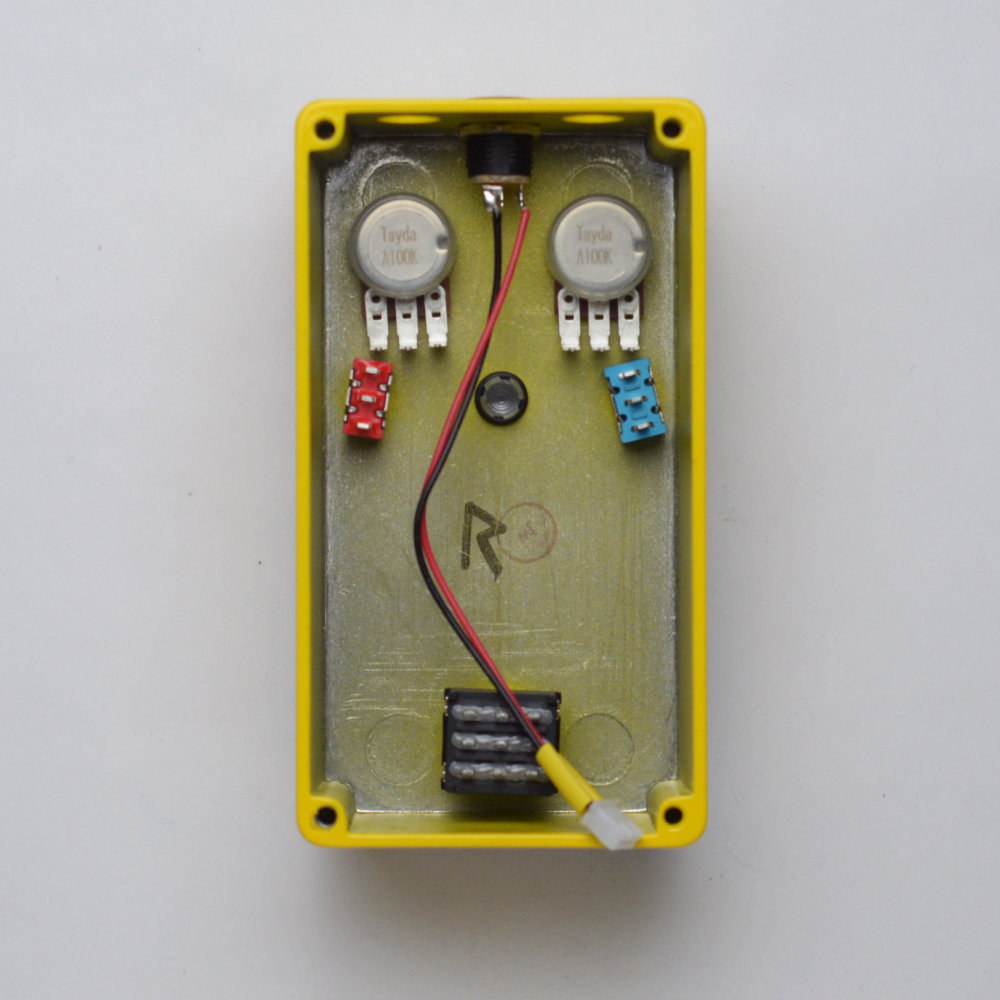
\includegraphics[width=\textwidth]{build/09-enclosure-mount-inside-1000px.jpg}
  \end{subfigure}
  \begin{subfigure}[b]{0.49\textwidth}
    \centering
    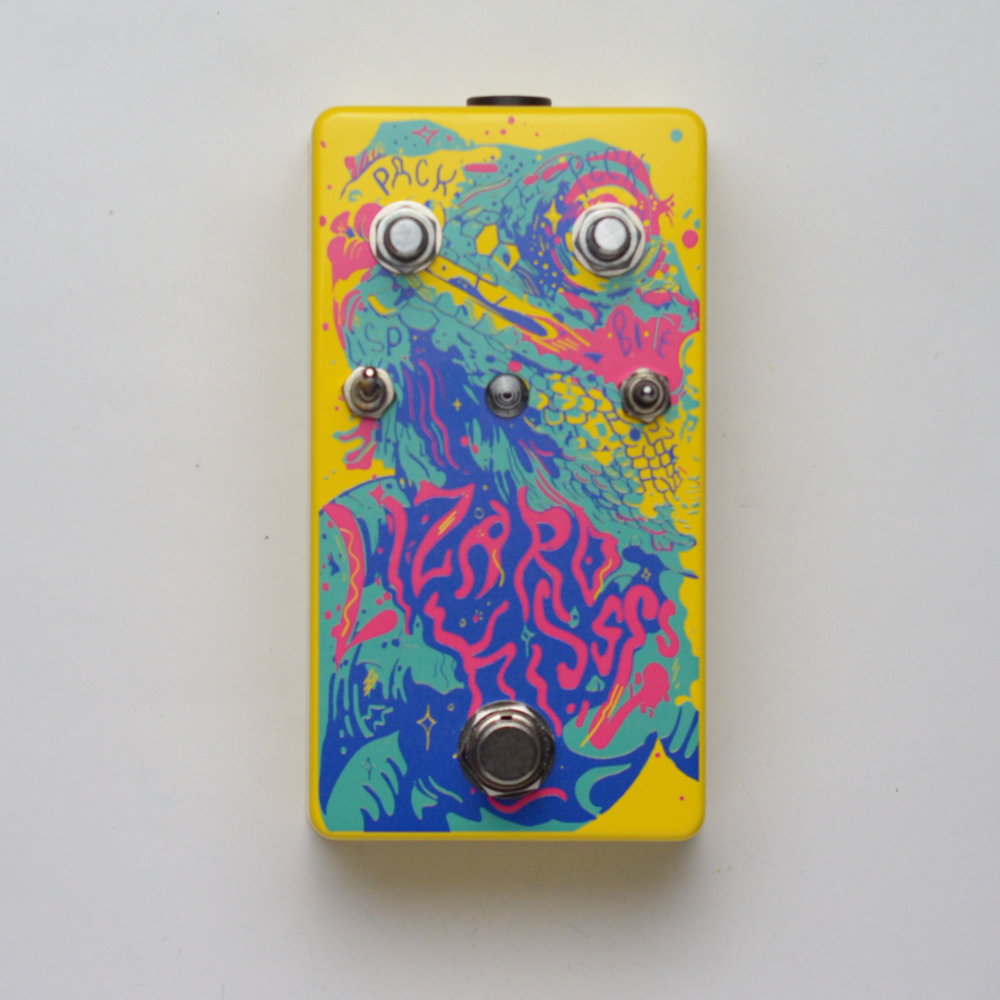
\includegraphics[width=\textwidth]{build/08-enclosure-mount-1000px.jpg}
  \end{subfigure}
  \caption{Inside and outside of the enclosure with parts
  mounted}
\end{figure}

\begin{figure}[h!]
  \centering
  \begin{subfigure}[b]{0.49\textwidth}
    \centering
    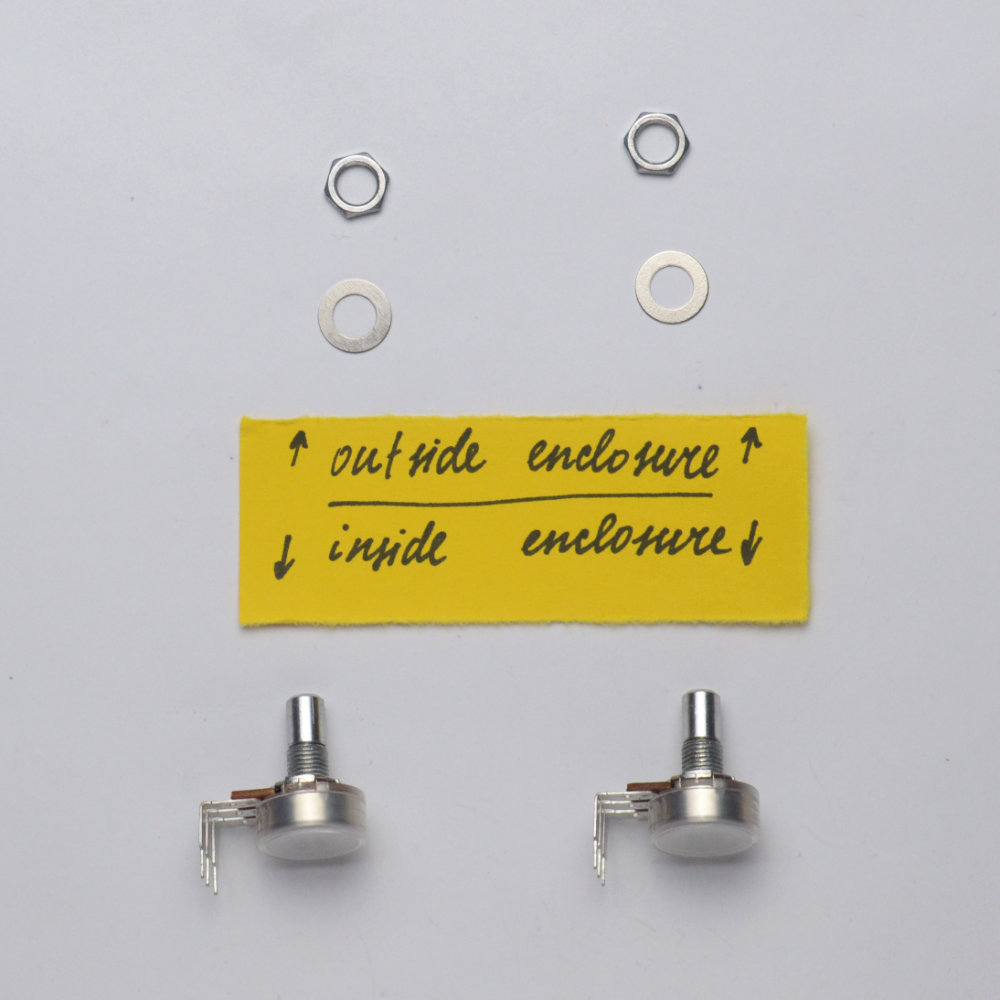
\includegraphics[width=\textwidth]{build/04-pots-mount-1000px.jpg}
  \end{subfigure}
  \begin{subfigure}[b]{0.49\textwidth}
    \centering
    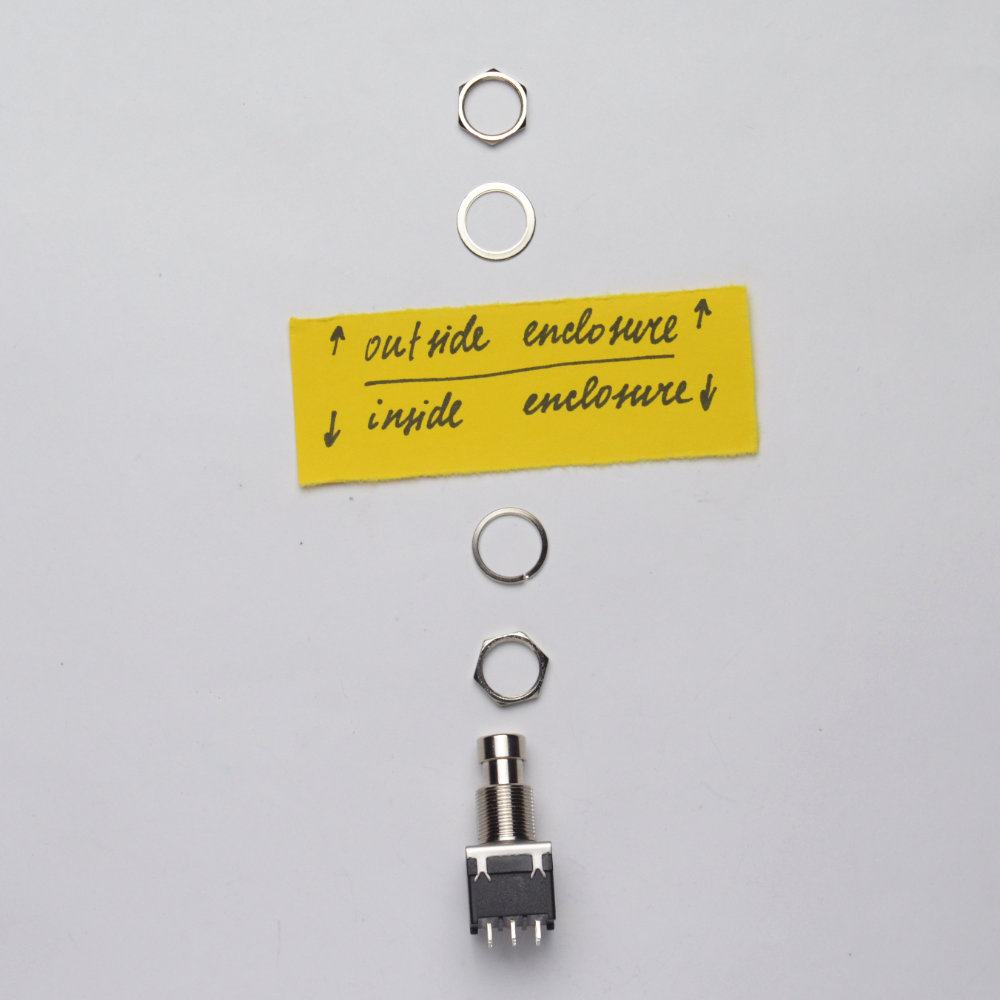
\includegraphics[width=\textwidth]{build/05-fs-mount-1000px.jpg}
  \end{subfigure}
  \caption{How to mount potentiometers and the footswitch}
\end{figure}

\begin{figure}[h!]
  \centering
  \begin{subfigure}[b]{0.49\textwidth}
    \centering
    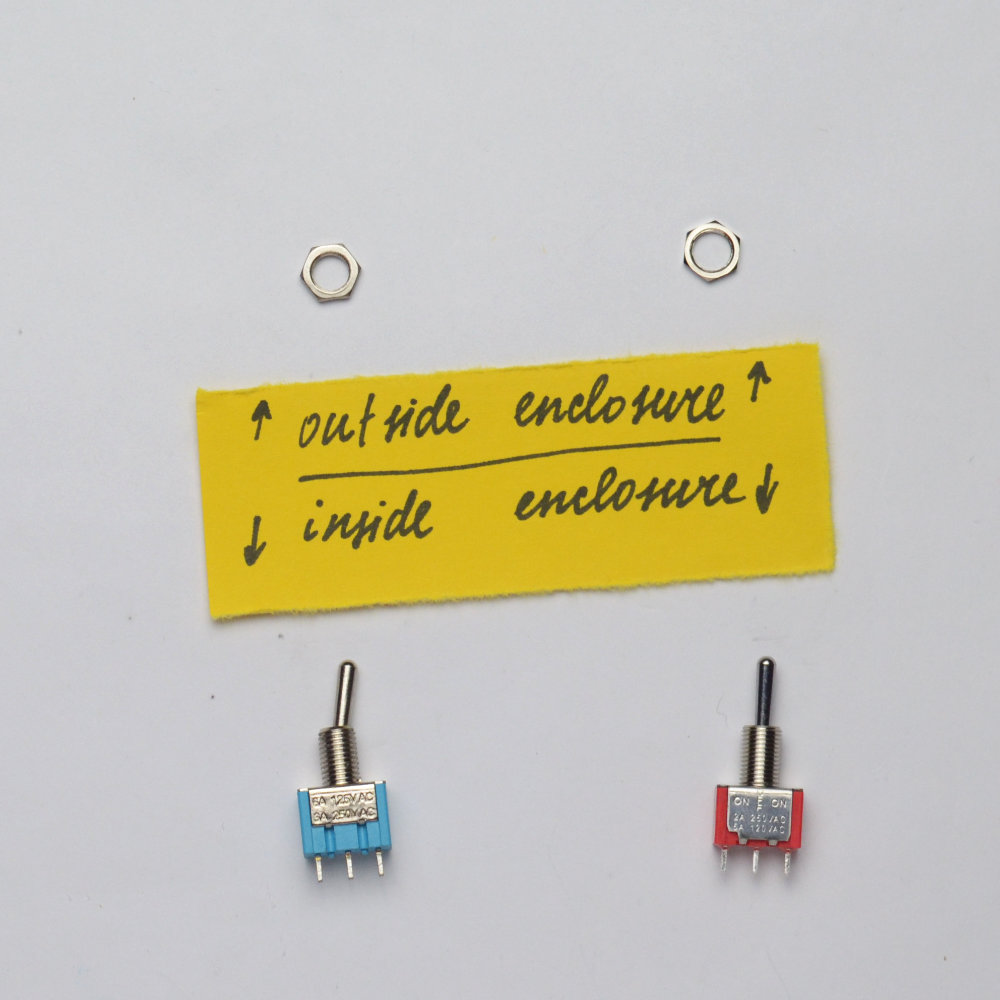
\includegraphics[width=\textwidth]{build/06-sw-mount-1000px.jpg}
  \end{subfigure}
  \begin{subfigure}[b]{0.49\textwidth}
    \centering
    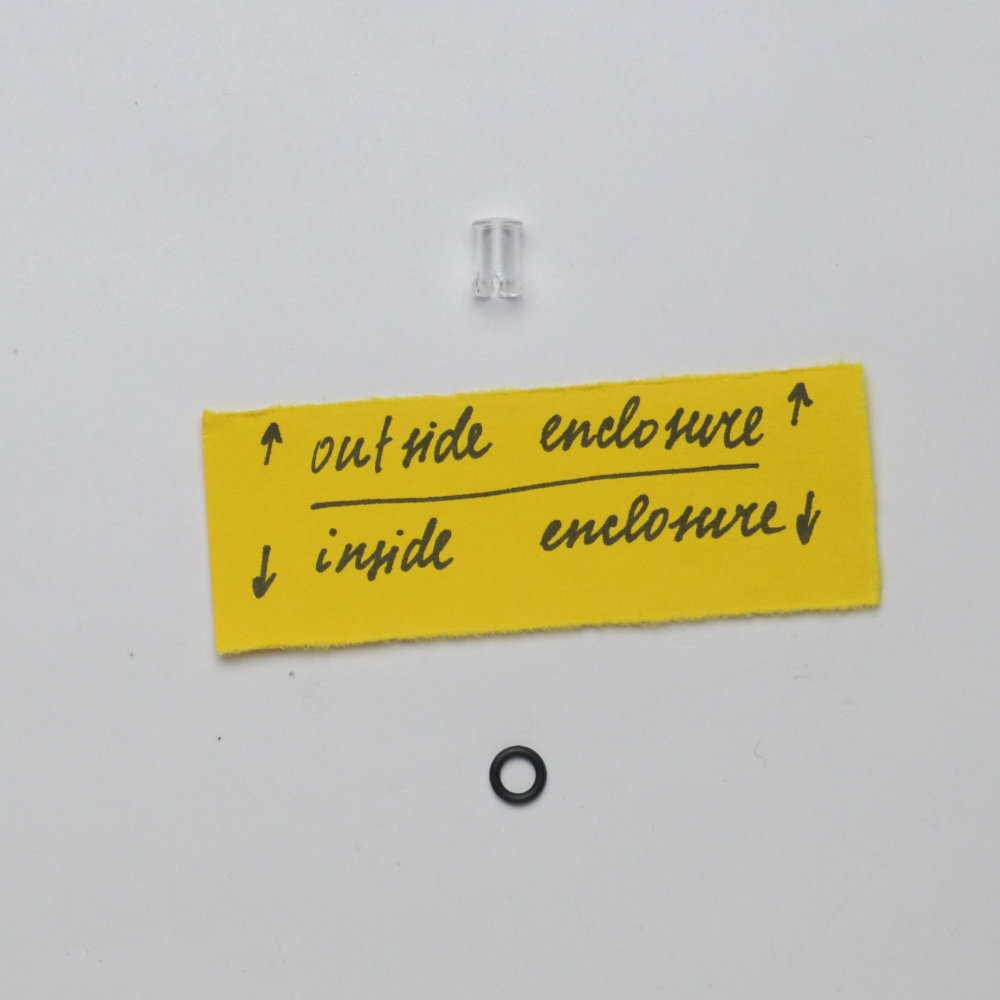
\includegraphics[width=\textwidth]{build/07-lampshade-mount-1000px.jpg}
  \end{subfigure}
  \caption{How to mount toggle switches and the lampshade}
\end{figure}

\restoregeometry{}

% \begin{figure}[h!]
%   \begin{center}
%     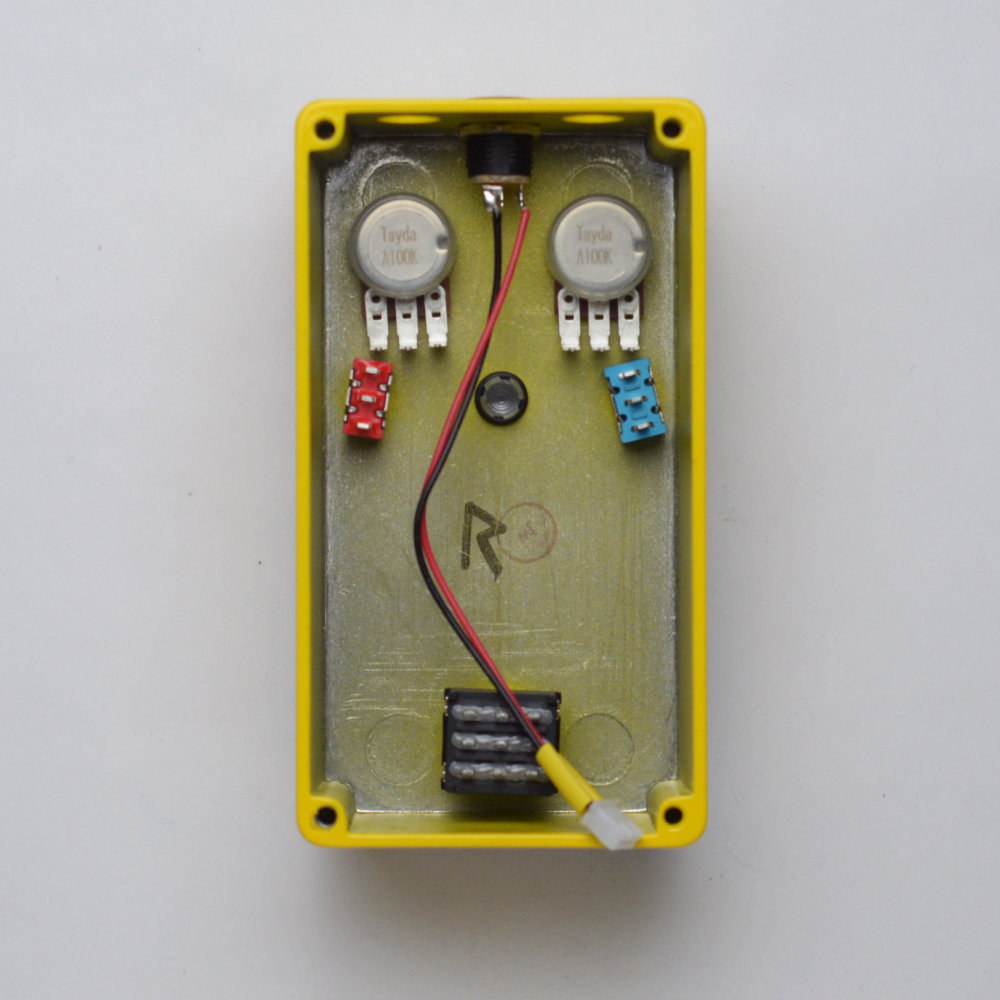
\includegraphics[width=0.7\textwidth]{build/09-enclosure-mount-inside-1000px.jpg}
%   \end{center}
%   \caption{Inside of the enclosure with parts mounted}
% \end{figure}


% \begin{figure}[h!]
%   \begin{center}
%     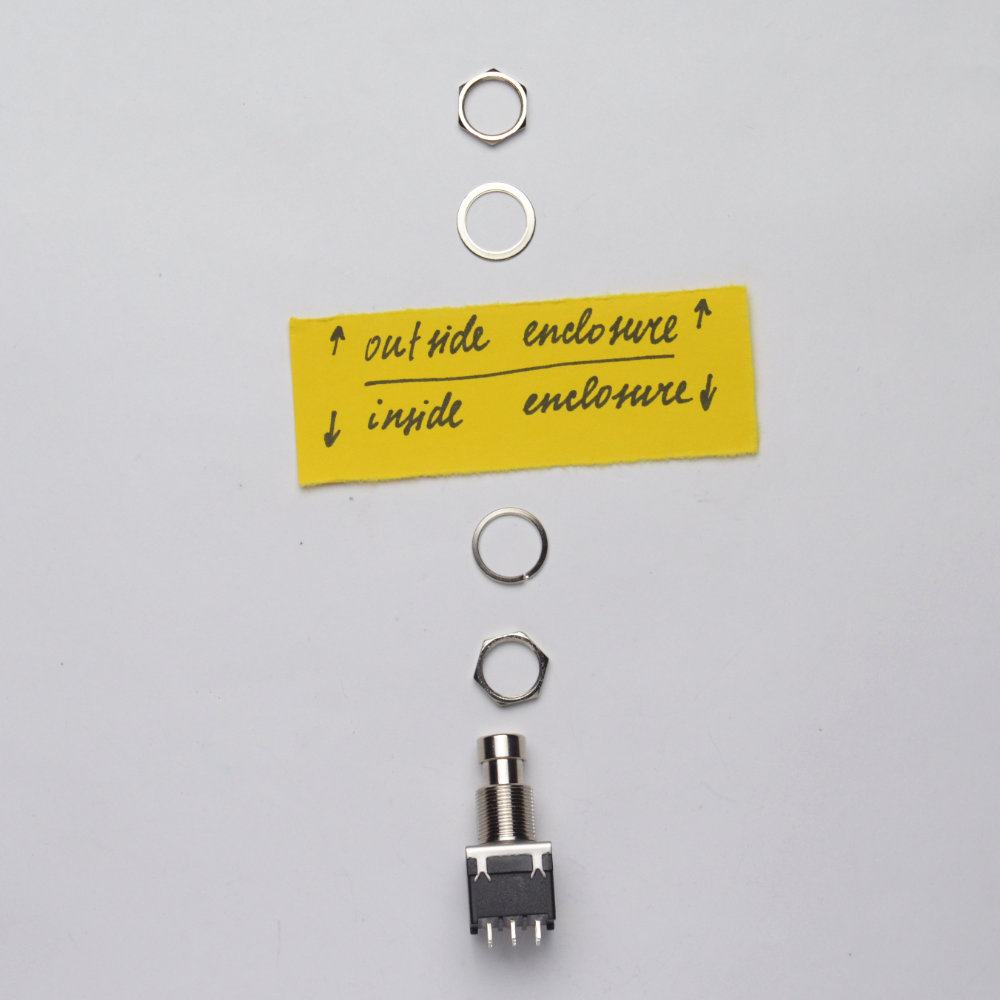
\includegraphics[width=0.5\textwidth]{build/05-fs-mount-1000px.jpg}
%   \end{center}
%   \caption{How to mount the footswitch}
% \end{figure}

% \begin{figure}[h!]
%   \begin{center}
%     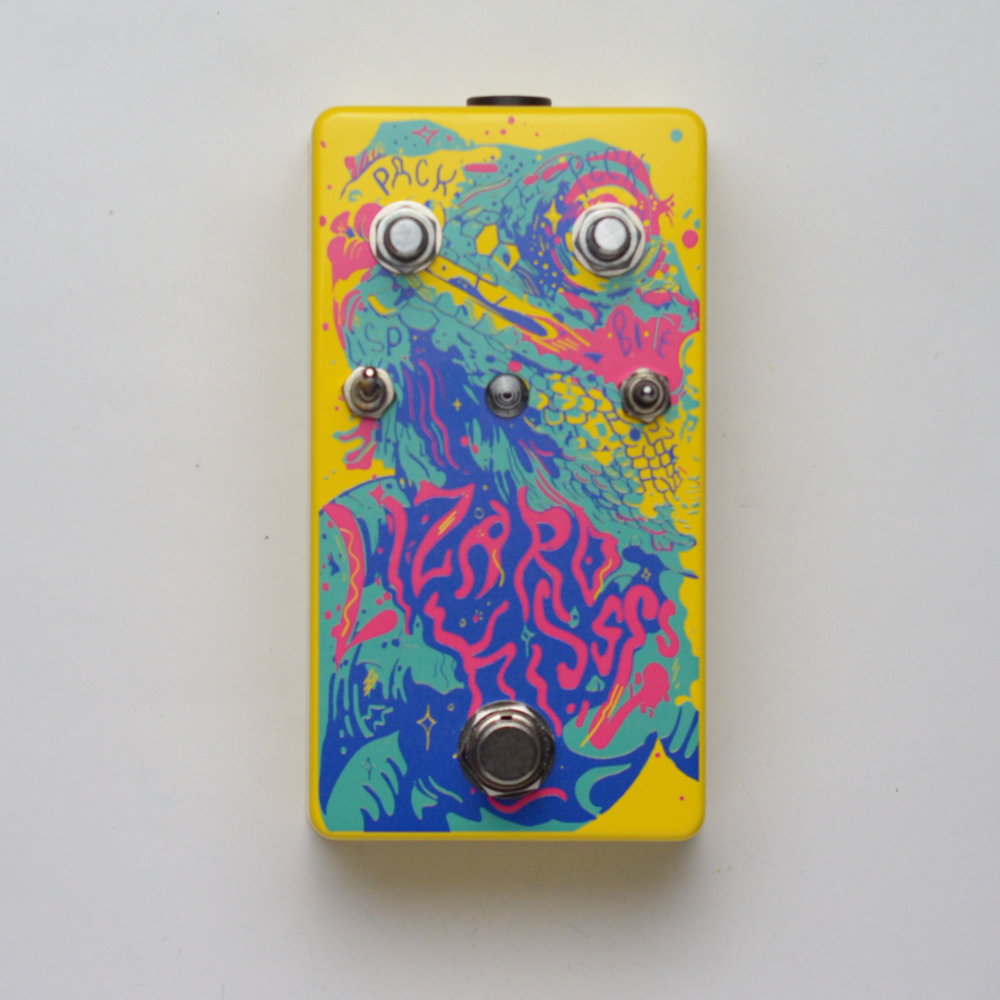
\includegraphics[width=0.7\textwidth]{build/08-enclosure-mount-1000px.jpg}
%   \end{center}
%   \caption{Outside of the enclosure with parts mounted}
% \end{figure}

\subsection{Populate Main Board}

\begin{itemize}
  \item Go through the \textbf{Main Board, floor side} section of the
    \hyperref[tbl:BOM]{BOM table} from top to bottom;
  \item One component at a time:
    \begin{itemize}
      \item Insert the part into the PCB;
      \item Flip the PCB and solder the part to the pads;
      \item Cut the excess component leads;
    \end{itemize}
\end{itemize}

\begin{figure}[h!]
  \centering
  \begin{subfigure}[b]{0.49\textwidth}
    \centering
    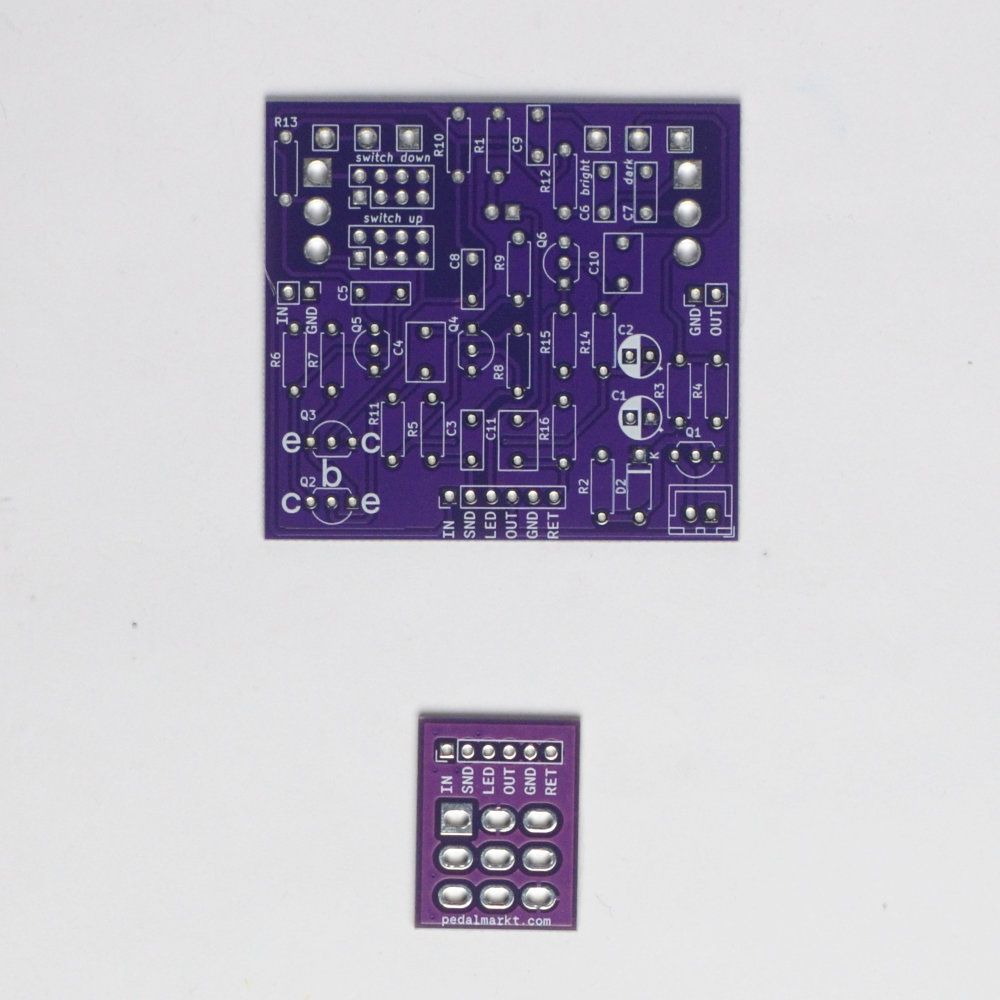
\includegraphics[width=\textwidth]{build/01-board-floor-1000px.jpg}
  \end{subfigure}
  \begin{subfigure}[b]{0.49\textwidth}
    \centering
    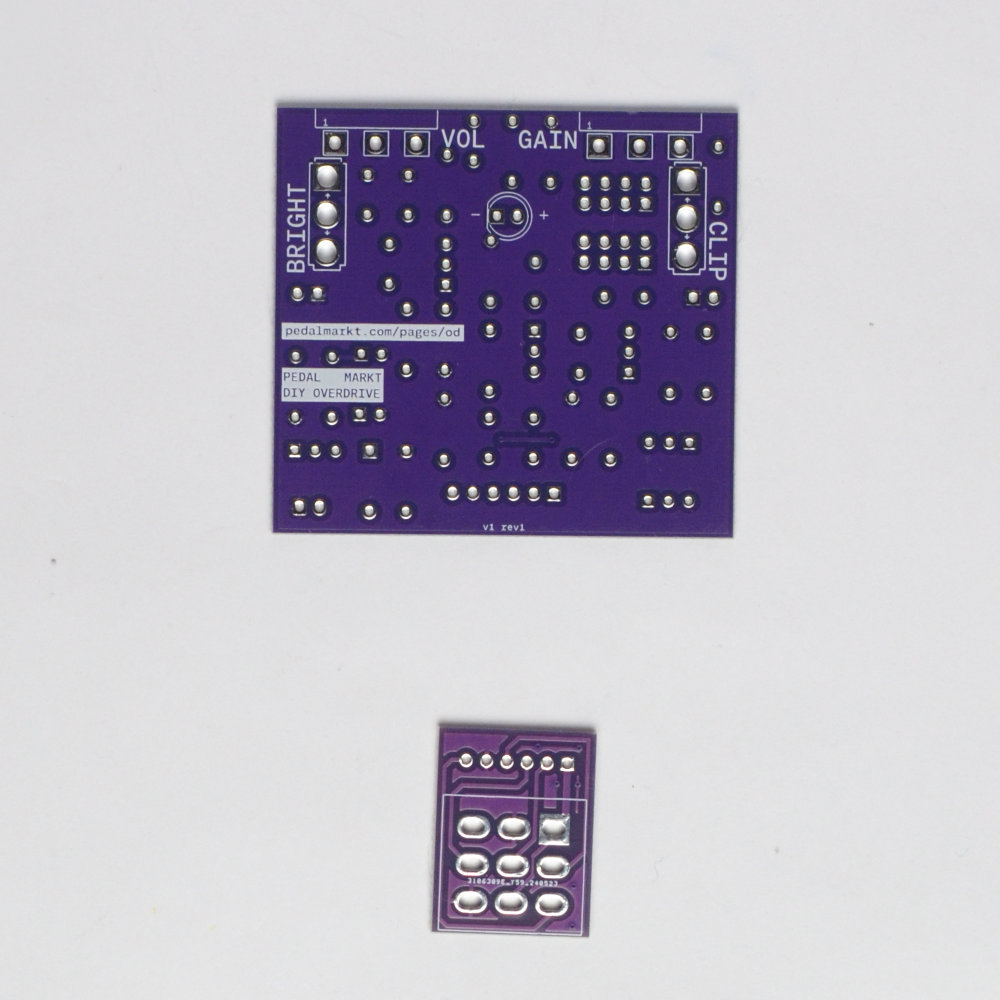
\includegraphics[width=\textwidth]{build/02-board-player-1000px.jpg}
  \end{subfigure}
  \caption{Main and switch boards, floor side on the left,
  player side on the right}
\end{figure}

\newgeometry{vmargin={3cm},hmargin={1cm}}

\begin{figure}[h!]
  \centering
  \begin{subfigure}[b]{0.49\textwidth}
    \centering
    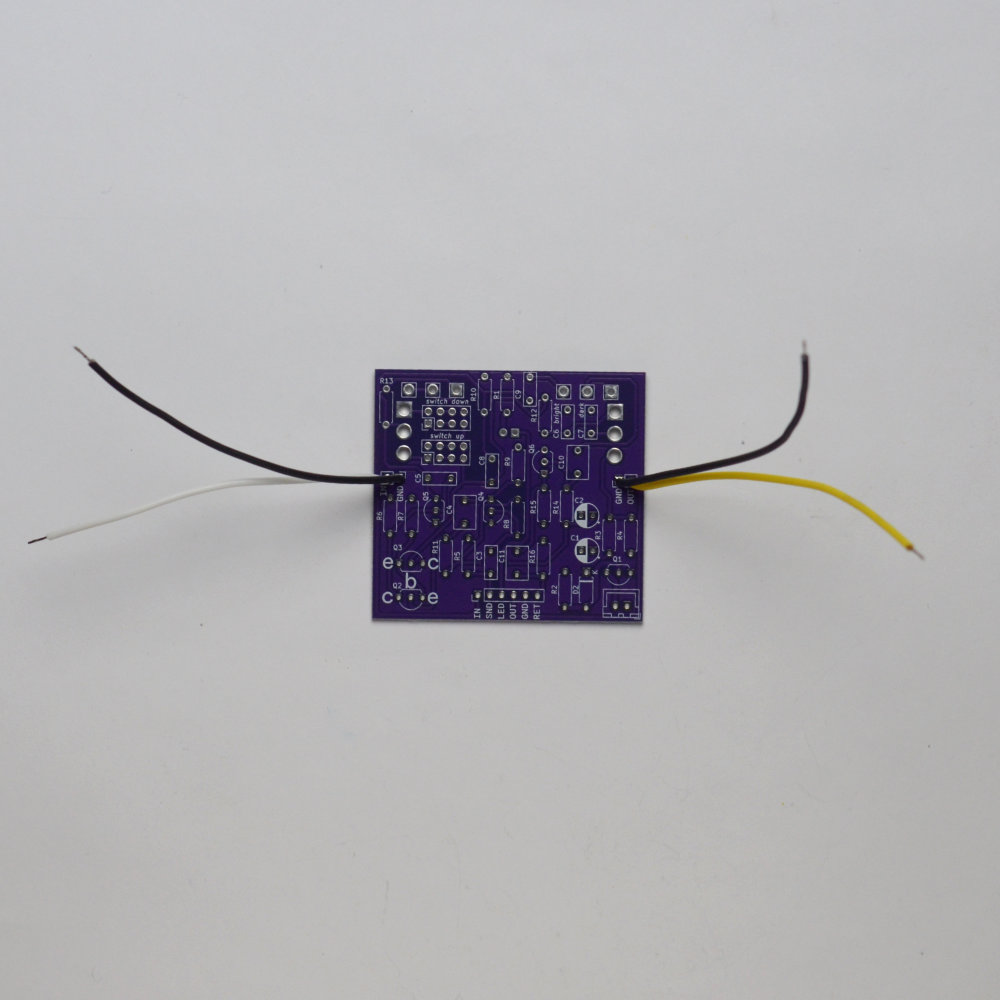
\includegraphics[width=\textwidth]{build/10-board-wires-1000px.jpg}
  \end{subfigure}
  \begin{subfigure}[b]{0.49\textwidth}
    \centering
    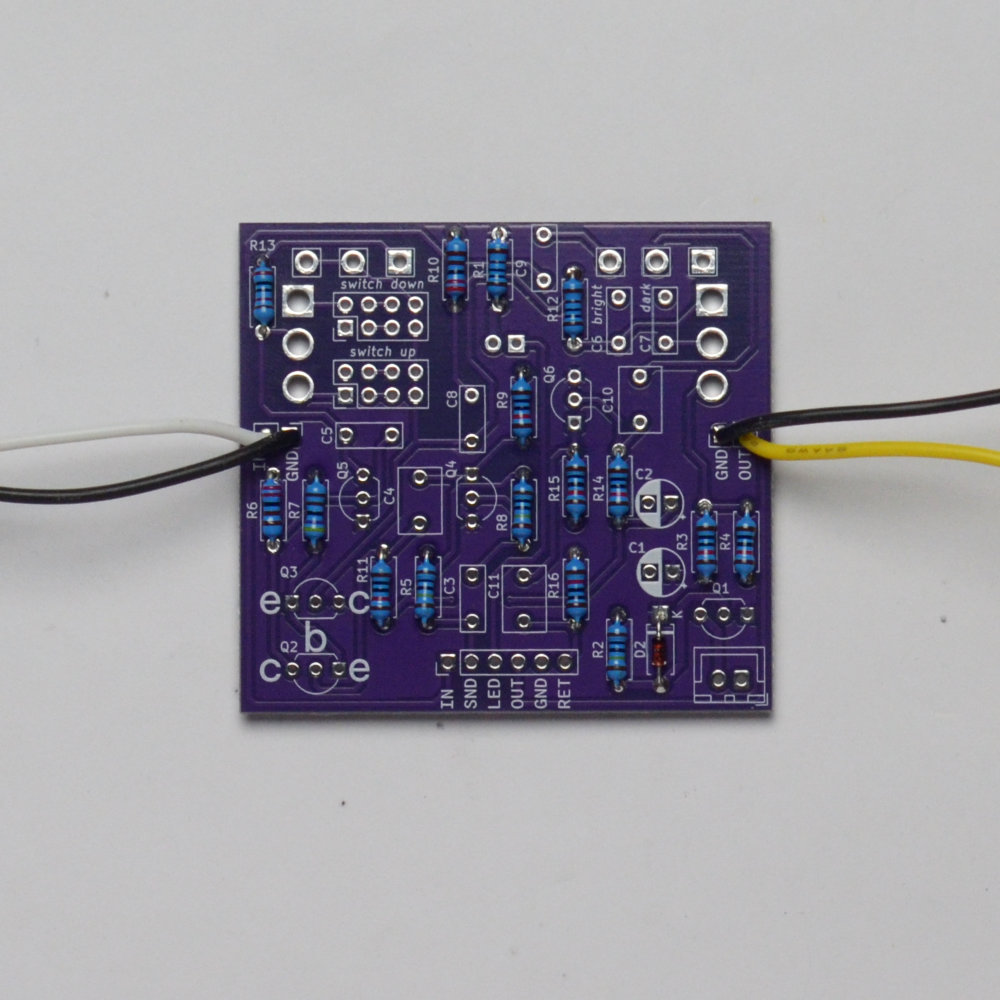
\includegraphics[width=\textwidth]{build/11-board-resistors-1000px.jpg}
  \end{subfigure}
  \caption{Wires soldered on the left, resistors on the right}
\end{figure}

\begin{figure}[h!]
  \centering
  \begin{subfigure}[b]{0.49\textwidth}
    \centering
    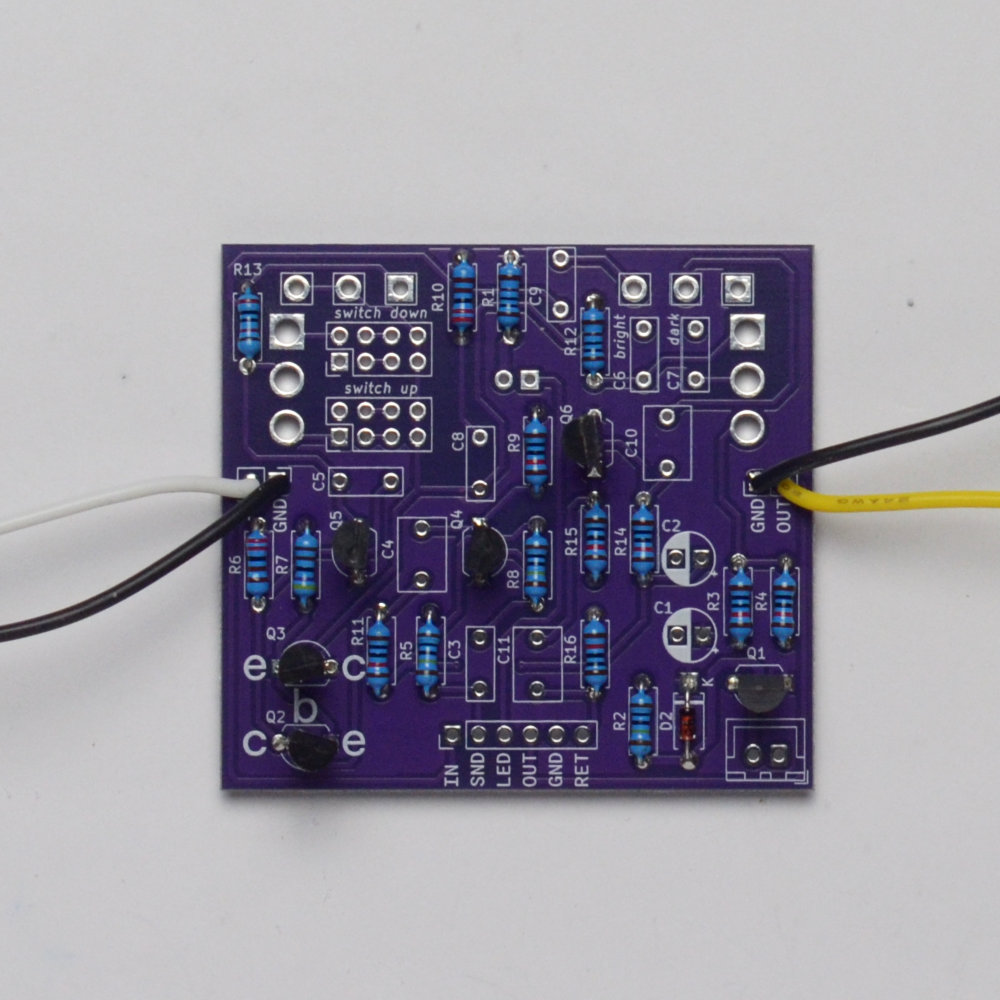
\includegraphics[width=\textwidth]{build/12-board-transistors-1000px.jpg}
  \end{subfigure}
  \begin{subfigure}[b]{0.49\textwidth}
    \centering
    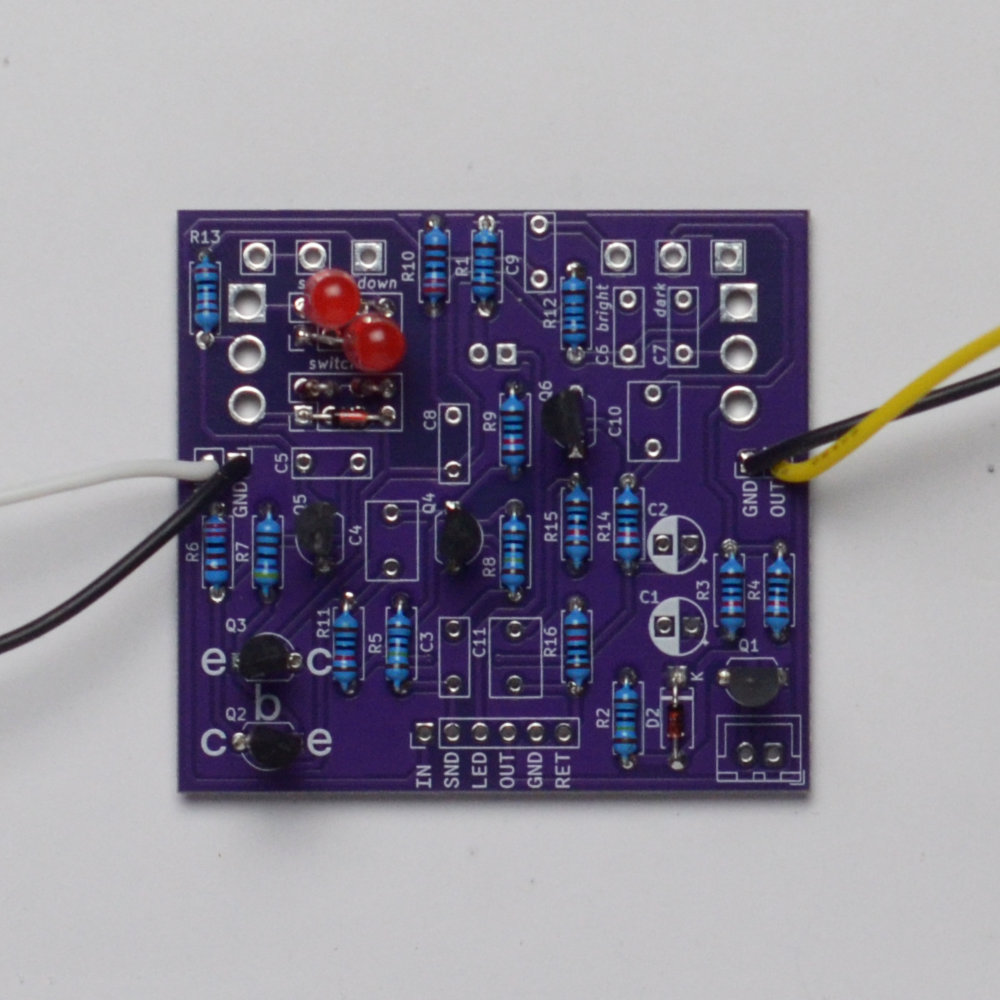
\includegraphics[width=\textwidth]{build/13-board-clipping-1000px.jpg}
  \end{subfigure}
  \caption{Transistors soldered on the left, diodes on the right}
\end{figure}

\begin{figure}[h!]
  \centering
  \begin{subfigure}[b]{0.49\textwidth}
    \centering
    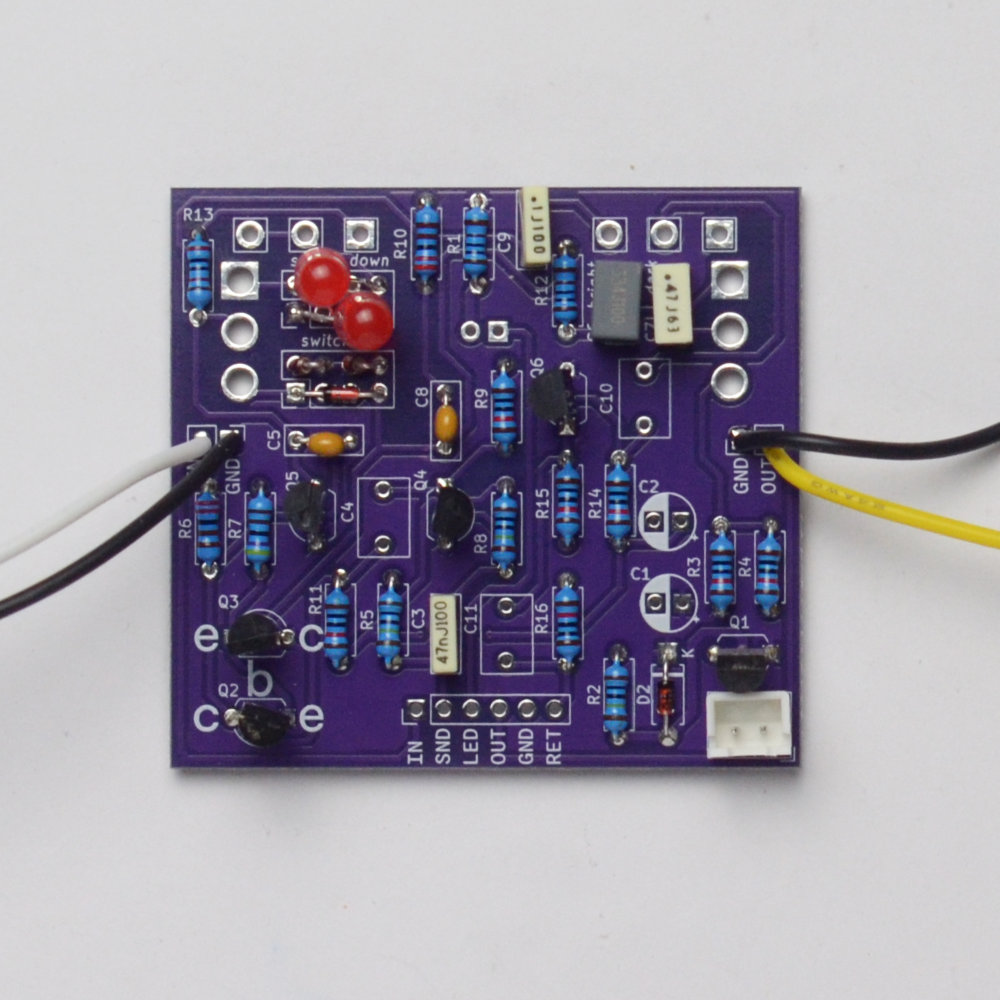
\includegraphics[width=\textwidth]{build/15-board-caps-1000px.jpg}
  \end{subfigure}
  \begin{subfigure}[b]{0.49\textwidth}
    \centering
    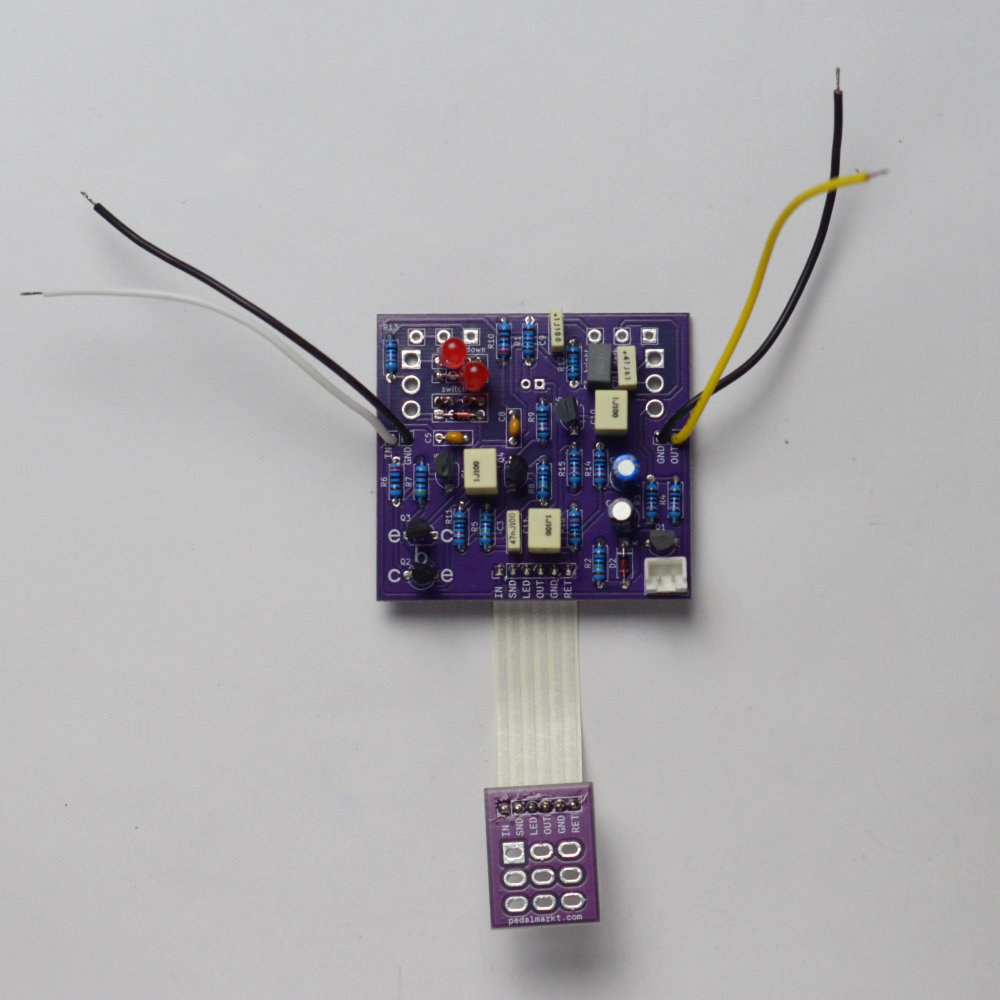
\includegraphics[width=\textwidth]{build/15-board-daughter-board-1000px.jpg}
  \end{subfigure}
  \caption{Caps soldered on the left, switch board and ribbon
  on the right}
\end{figure}


\restoregeometry{}

\subsection{Solder Jacks and LED}

\begin{itemize}
  \item Solder audio jacks to the wires coming from the Main
    Board. Black (GND) wire should be connected to the lug
    that is connected to the round part on the inside of the
    jack socket. The colored wire (IN or OUT) should be
    connected to the other lug.
  \item Place the LED into the pads \textbf{on the player
    side} of the board. The short leg of the LED should go
    into the "-" (minus) pad. Do not solder the LED just
    yet.
\end{itemize}

\begin{figure}[h!]
  \centering
  \begin{subfigure}[b]{0.49\textwidth}
    \centering
    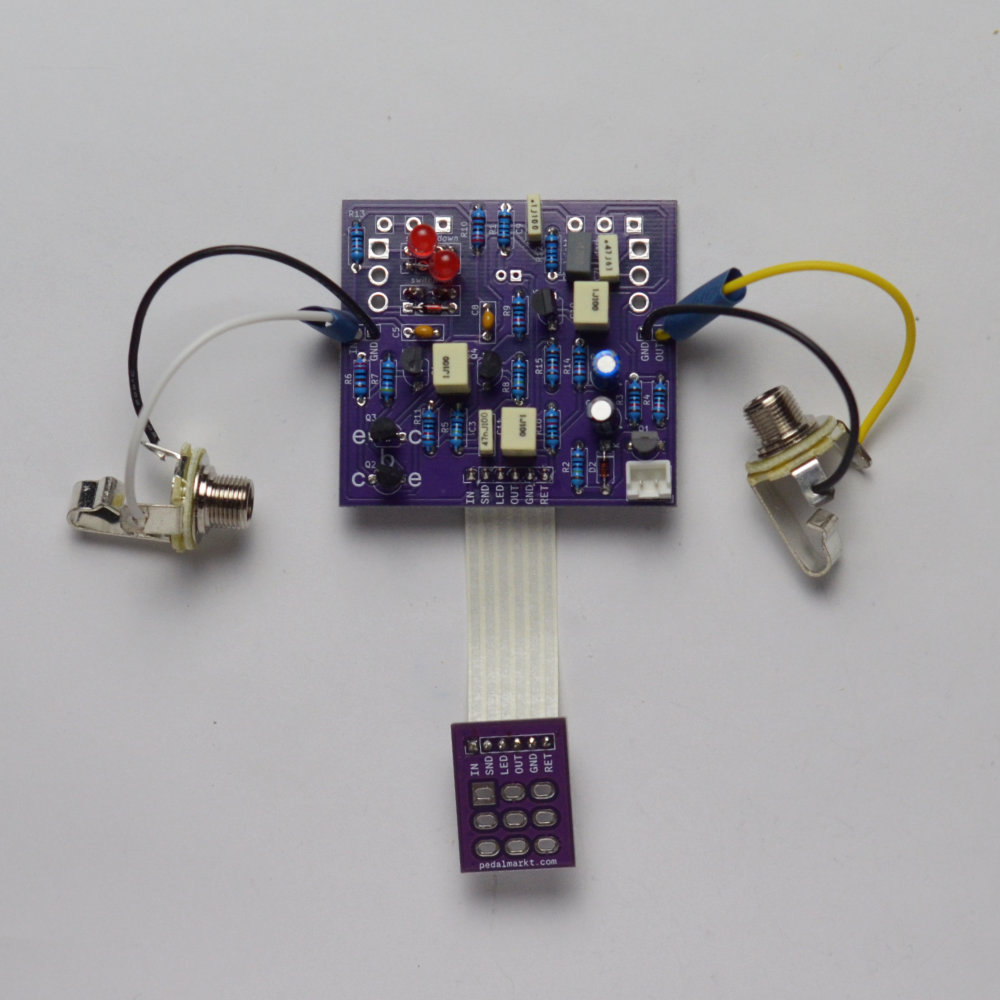
\includegraphics[width=\textwidth]{build/17-board-jacks-1000px.jpg}
  \end{subfigure}
  \begin{subfigure}[b]{0.49\textwidth}
    \centering
    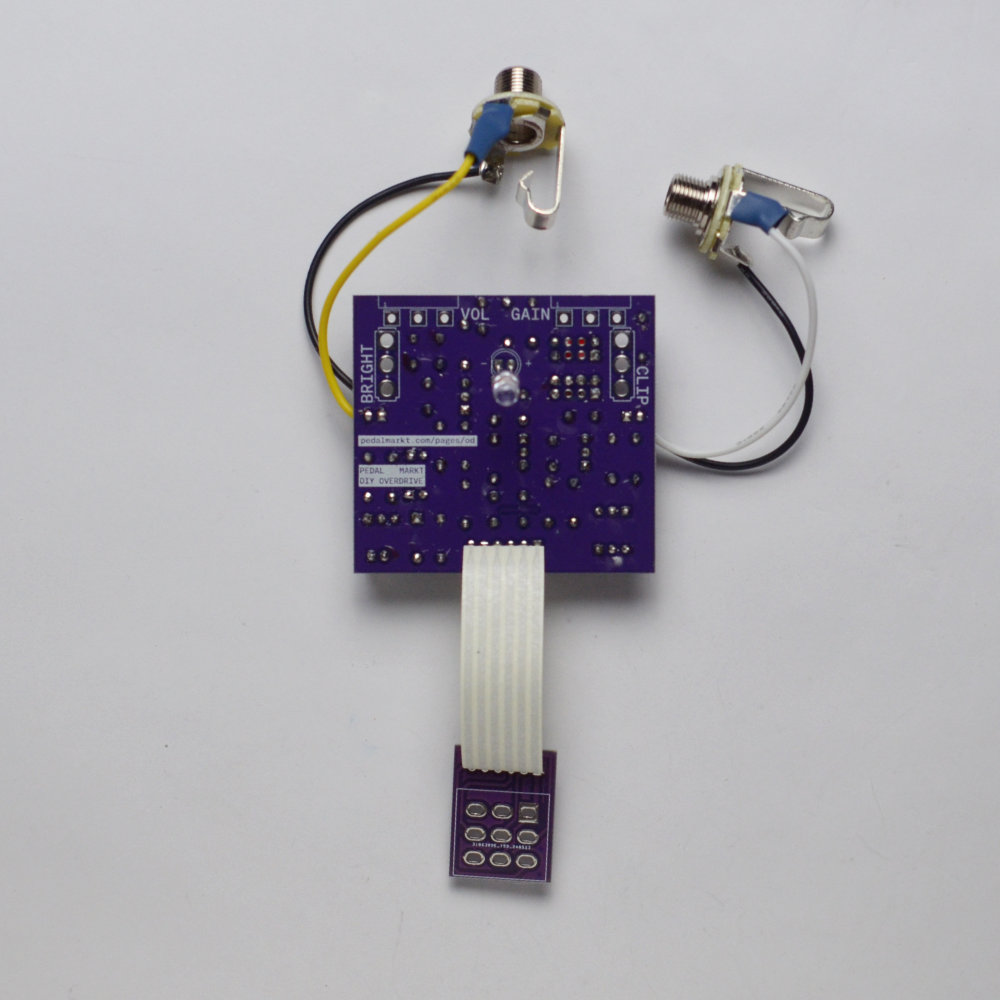
\includegraphics[width=\textwidth]{build/18-board-jacks-player-1000px.jpg}
  \end{subfigure}
  \caption{Audio jacks soldered on the left, LED placed but
  not soldered on the right}
\end{figure}

\pagebreak

\subsection{Mount boards into enclosure}

\begin{itemize}
  \item Place the main board into the enclosure, floor side
    of the board facing you;
    \begin{itemize}
      \item Make sure all the legs of the potentiometers and toggle
        switches get inserted into their dedicated pads;
      \item Make sure the LED gets inserted into the
        lampshade. You might have to press on the lampshade
        from the other side of the enclosure so that it
        doesn't lift from the enclosure;
      \item Solder the pots, the toggle switches and the LED to
        the main board;
    \end{itemize}
  \item Place the switch board onto the footswitch and
    solder them together.
\end{itemize}


\begin{figure}[h!]
  \begin{center}
    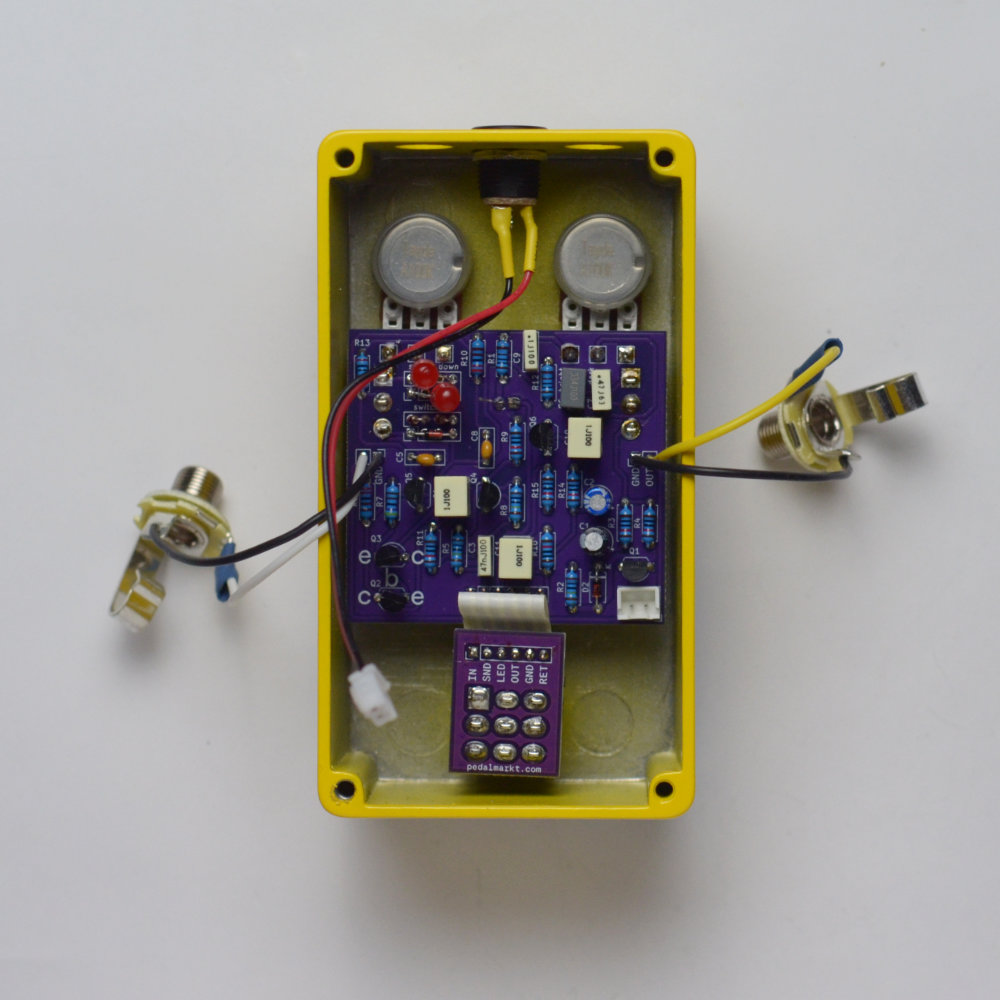
\includegraphics[width=0.8\textwidth]{build/19-board-enclosure-1000px.jpg}
  \end{center}
  \caption{Inside of the enclosure with boards mounted}
\end{figure}

\pagebreak

\subsection{Complete the pedal}

\begin{itemize}
  \item Mount the audio jacks onto the enclosure;
  \item Connect the DC cable to the socket on the bottom
    right of the board;
  \item Plug in and test the pedal!
\end{itemize}


\begin{figure}[h!]
  \begin{center}
    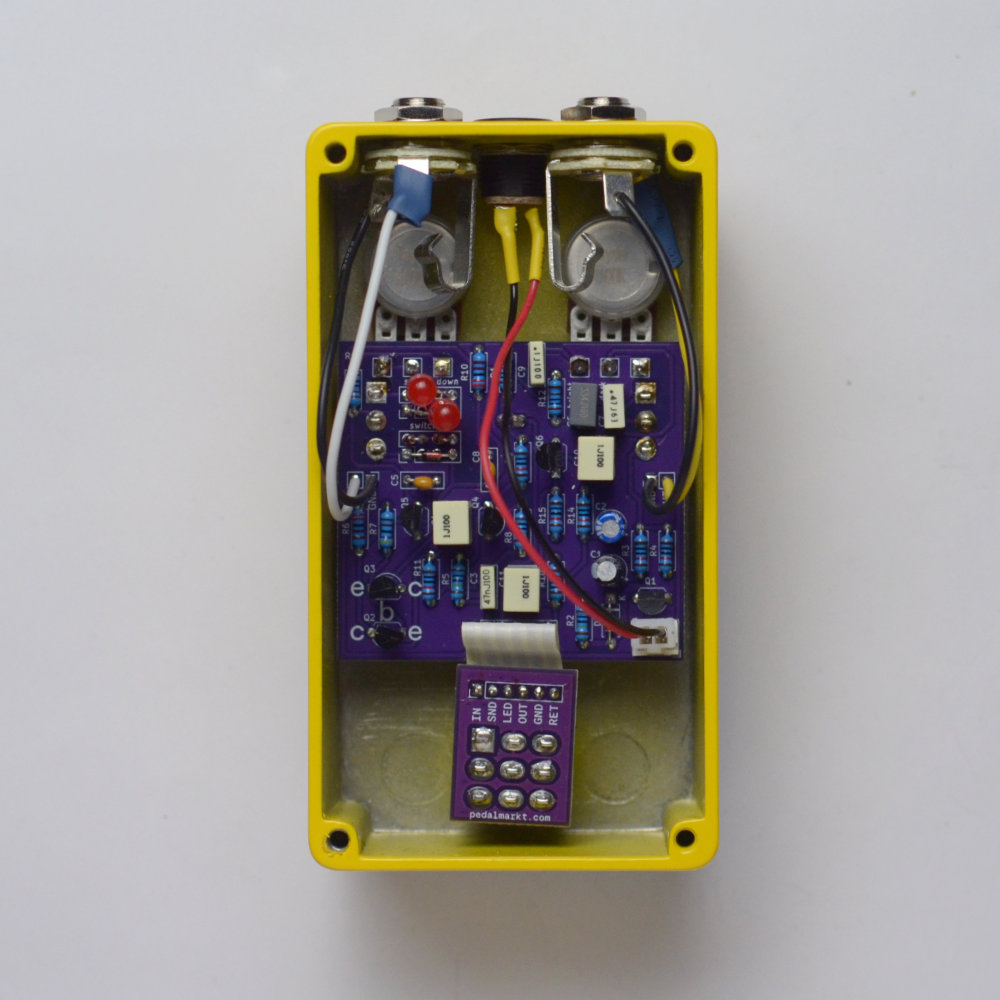
\includegraphics[width=\textwidth]{build/20-built-1000px.jpg}
  \end{center}
  \caption{Built pedal}
\end{figure}

\pagebreak

\section{Schematic}
\label{sec:schematic}

\section{Circuit breakdown}
\label{sec:circuit}
\end{document}
